Nachdem wir uns in dieser Arbeit hauptsächlich mit dem WIE \ac{qc} die aktuelle asymmetrische Kryptografie brechen können und wie mit diesem Problem auf einer technischen Ebene umgegangen werden kann, gilt es noch eine weitere Frage zu beantworten. Warum müssen wir uns schon jetzt mit dieser potentiellen Gefahr auseinandersetzen? Ein großteil der vorgestellen Konzepte und Algorithmen sind nur theoretischer Natur und aktuelle \ac{qc} sind nicht in der Lage zum Beispiel RSA zu decodieren. Warum also hat das NIST seine Ausschreibung für einen Quantensichern Algorithmus gestartet? Warum sollte die Gefahr eines \ac{qc}s auf die Kryptographie schon jetzt ernst genommen werden?\\
Zum einen gilt es die Frage zu beantworten wann es  wahrscheinlich es ist, dass ein \ac{qc} in der Lage ist eine mit RSA-2048 bit verschlüsselte Nachricht zu entschlüsseln. Das theoretische minimum an benötigte Qbits hierfür liegt laut Abschätzungen der Schweizer IT-Sicherheitsfirma \textit{Kudelski Security} bei 6190 logischen Qbits \cite{gagliardoni_quantum_2021}. Dies berücksichtigt jedoch Faktoren wie Implementierungs-Details und Fehlerkorrektur nicht. Einer anderen Schätzung zufolge würden eher um die 10.000 reale Qbits benötigt\cite{ziegler_online_2015}. Wie Lange wird es dauern bis ein \ac{qc} mit einer solchen Anzahl an Qbits Realität ist?\\
Schaut man auf die \textit{Timeline} der Firma IBM (siehe Grafik \ref{fig:ibm-rm}) so sieht man, dass der aktuelle entwicklungsstand ein \ac{qc} mit 433 Qbits ist. Dies stellt schon ein enormes Wachstum zu den 27 Qbits in 2019 dar. Der Plan ist es bis 2025 auf ungefähr 4000 Qbits zu gelangen und nach 2026 10.000 und mehr Qbits anzupeilen \cite{noauthor_ibm_2015}.\\
Diese Vorhersage deckt sich auch mit den Ansichten führende Experten in dem Gebiet der Quantenkryptografie. Bei einer Befragung des \textit{Global Risk Intites} an der 47 Forschende teilnahmen ergab sich die folgenden Ergebnisse. Es wird für sehr wahrscheinlich gehalten, dass in den nächsten 15 bis 20 Jahren ein \ac{qc} in der Lage sein wird RSA-2048 zu brechen mindestens aber in 30 Jahren soll dies mit nahezu vollständiger Sicherheit möglich sein \cite{noauthor_2021_nodate}.

\begin{figure}[!hbt]
    \centering
    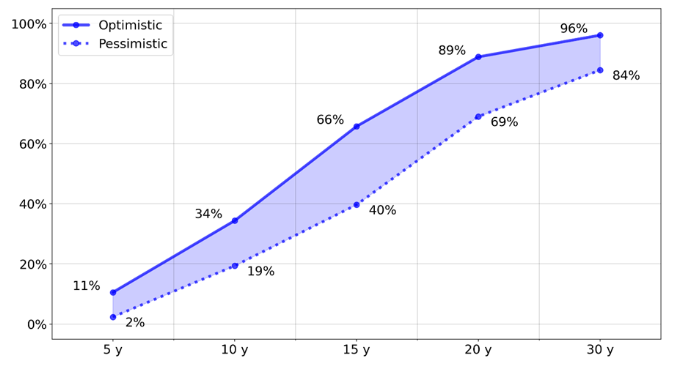
\includegraphics[width=0.5\textwidth]{images/estiamte-qc.png}
    \caption{Wahrscheinlichkeit wann laut Experten des Quantencomputing RSA-2048 durch einen \ac{qc} gebrochen sein kann \cite{noauthor_2021_nodate}}
    \label{fig:qx-approx}
\end{figure}\

Wenn 